\documentclass[11pt]{article}

% Change "review" to "final" to generate the final (sometimes called camera-ready) version.
% Change to "preprint" to generate a non-anonymous version with page numbers.
% \usepackage[review]{acl}
\usepackage[final]{acl}

% Standard package includes
\usepackage{times}
\usepackage{latexsym}

% For proper rendering and hyphenation of words containing Latin characters (including in bib files)
\usepackage[T1]{fontenc}
% For Vietnamese characters
% \usepackage[T5]{fontenc}
% See https://www.latex-project.org/help/documentation/encguide.pdf for other character sets

% This assumes your files are encoded as UTF8
\usepackage[utf8]{inputenc}

% This is not strictly necessary, and may be commented out,
% but it will improve the layout of the manuscript,
% and will typically save some space.
\usepackage{microtype}

% This is also not strictly necessary, and may be commented out.
% However, it will improve the aesthetics of text in
% the typewriter font.
\usepackage{inconsolata}

%Including images in your LaTeX document requires adding
%additional package(s)
\usepackage{graphicx}


\usepackage{amsmath}
\usepackage{amssymb}
\usepackage{subfigure}
\usepackage{booktabs}
\usepackage{multirow}
\usepackage{makecell}

% If the title and author information does not fit in the area allocated, uncomment the following
%
%\setlength\titlebox{<dim>}
%
% and set <dim> to something 5cm or larger.

%%%%%

\def\tightlist{} % ignore this command

\title{Learning to Refer: How Scene Complexity Affects Emergent Communication in Neural Agents}

% Author information can be set in various styles:
% For several authors from the same institution:
% \author{Author 1 \and ... \and Author n \\
%         Address line \\ ... \\ Address line}
% if the names do not fit well on one line use
%         Author 1 \\ {\bf Author 2} \\ ... \\ {\bf Author n} \\
% For authors from different institutions:
% \author{Author 1 \\ Address line \\  ... \\ Address line
%         \And  ... \And
%         Author n \\ Address line \\ ... \\ Address line}
% To start a seperate ``row'' of authors use \AND, as in
% \author{Author 1 \\ Address line \\  ... \\ Address line
%         \AND
%         Author 2 \\ Address line \\ ... \\ Address line \And
%         Author 3 \\ Address line \\ ... \\ Address line}

\author{Dominik Künkele$^{1}$ \and Simon Dobnik$^{1,2}$ \\
        Department of Philosophy, Linguistics and Theory of Science$^{1}$ \\ 
        Centre for Linguistic Theory and Studies in Probability (CLASP)$^{2}$ \\
        University of Gothenburg, Sweden \\
        \texttt{contact@dominik-kuenkele.de} \and \texttt{simon.dobnik@gu.se}}

\begin{document}

\maketitle
\begin{abstract}
  We explore how neural network-based agents learn to map continuous sensory input to discrete linguistic symbols through interactive language games.
  One agent describes objects in 3D scenes using invented vocabulary; the other interprets references based on attributes.
  We extend the CLEVR dataset with more complex scenes to study how increased referential complexity impacts language acquisition and symbol grounding in artificial agents.
\end{abstract}
% Here's a \textbf{\textasciitilde2000-word summary} of the paper you
% provided, which explores how artificial neural agents develop
% referential communication in visually grounded environments:

% \textbf{Summary of the Paper on Emergent Referential Communication in
% Neural Agents}

% \textbf{1. Introduction and Motivation}

% The paper addresses the \textbf{symbol grounding problem}---how
% cognitive or artificial systems connect \textbf{continuous sensory
% input} (like vision) with \textbf{discrete symbolic representations}
% (like language). This challenge is central to building AI systems that
% can understand and use language meaningfully in the real world.

% A key focus is on \textbf{referring expressions}---linguistic phrases
% that uniquely identify objects in a scene. The authors build on the
% \textbf{Dale and Reiter (1995)} algorithm, which incrementally adds
% attributes to descriptions until the target object is uniquely
% identified. The study investigates how \textbf{neural agents} can learn
% to generate and interpret such expressions through \textbf{language
% games}, where communication protocols emerge from interaction rather
% than being pre-programmed.

% \textbf{2. Dataset Design}

% To study this, the authors extend the \textbf{CLEVR dataset}, a
% synthetic visual dataset designed for reasoning tasks. They generate
% three new datasets with increasing complexity:

% \begin{itemize}
% \tightlist
% \item
%   \textbf{CLEVR Color}: The target object is uniquely identifiable by
%   color alone. Shape and size are shared with distractors.
% \item
%   \textbf{Dale-2}: One target and one distractor. The target is uniquely
%   identifiable by a minimal combination of attributes (color, shape,
%   size).
% \item
%   \textbf{Dale-5}: One target and four distractors. The target may share
%   multiple attributes with distractors, requiring more complex referring
%   expressions.
% \end{itemize}

% Each image contains up to 10 non-overlapping objects, and the datasets
% are designed to mimic the structure of natural language referring
% expressions.

% \textbf{3. Methodology}

% \textbf{Image Processing}

% Images are processed using a \textbf{ResNet-101} model followed by
% convolutional layers to extract feature maps. These features are used by
% the agents to generate or interpret messages.

% \textbf{Language Games Framework}

% The experiments use the \textbf{EGG (Emergence of Language in Games)}
% framework. Two agents---a \textbf{sender} and a
% \textbf{receiver}---communicate through a discrete channel:

% \begin{itemize}
% \tightlist
% \item
%   The \textbf{sender} sees the target object and generates a message
%   using an LSTM.
% \item
%   The \textbf{receiver} sees the full scene and interprets the message
%   to identify the target.
% \end{itemize}

% To enable backpropagation through discrete messages, the
% \textbf{Gumbel-Softmax} trick is used.

% \textbf{Attention Prediction Task}

% The receiver must predict a \textbf{3×3 region} around the target object
% in a \textbf{14×14 grid} over the image. The model outputs a probability
% distribution over regions, and performance is measured by the
% \textbf{probability mass} assigned to the correct region.

% \textbf{4. Experiments and Results}

% \textbf{Language Game Performance}

% The agents are trained on 128,000 games across different configurations
% of \textbf{message length (n)} and \textbf{vocabulary size (V)}. Key
% findings:

% \begin{itemize}
% \tightlist
% \item
%   \textbf{Dale-2}: Most configurations outperform the baseline (random
%   sender), with top models achieving over \textbf{96\% probability
%   mass}.
% \item
%   \textbf{Dale-5}: Only 8 out of 30 configurations beat the baseline.
%   Best models reach \textbf{84\%}, but many struggle due to increased
%   complexity.
% \item
%   \textbf{CLEVR Color}: Only two configurations outperform the baseline,
%   achieving \textbf{64--68\%}. Many configurations perform worse,
%   indicating that communication can sometimes mislead the receiver.
% \end{itemize}

% \textbf{Optimal configurations} tend to have \textbf{medium-sized
% vocabularies (V = 10--16)} and \textbf{message lengths (n = 3--4)}. Too
% few symbols limit expressiveness; too many hinder learning.

% \textbf{Error Analysis}

% Errors often occur when:

% \begin{itemize}
% \tightlist
% \item
%   The \textbf{target object is cropped out} during preprocessing.
% \item
%   The \textbf{receiver is confused} by distractors sharing multiple
%   attributes with the target.
% \item
%   The \textbf{message is too ambiguous}, especially in complex scenes.
% \end{itemize}

% \textbf{5. Natural Language Experiments}

% To better understand the agents' capabilities, the authors conduct two
% additional experiments using \textbf{natural language referring
% expressions} instead of emergent symbols.

% \textbf{Referring Expression Generation (Sender)}

% The sender is trained to generate expressions like ``small red cube''
% using the \textbf{Dale-Reiter GRE algorithm} as ground truth.
% Performance is evaluated using \textbf{accuracy, precision, and recall}.

% \begin{itemize}
% \tightlist
% \item
%   \textbf{Dale-2}: 99\% accuracy, near-perfect precision and recall.
% \item
%   \textbf{Dale-5}: 69\% accuracy, with lower scores for size attributes.
% \item
%   \textbf{CLEVR Color}: 93\% accuracy, perfect shape prediction, but
%   some color confusion.
% \end{itemize}

% \textbf{Size} is the hardest attribute to predict, followed by
% \textbf{color}, while \textbf{shape} is easiest. This suggests that
% \textbf{neural models struggle with attributes that are less visually
% salient or more context-dependent}.

% \textbf{Referring Expression Resolution (Receiver)}

% The receiver is trained to interpret natural language expressions and
% identify the correct region in the image.

% \begin{itemize}
% \tightlist
% \item
%   \textbf{Dale-2}: 95.16\% probability mass.
% \item
%   \textbf{Dale-5}: 92.19\%.
% \item
%   \textbf{CLEVR Color}: 95.33\%.
% \end{itemize}

% Interestingly, the receiver performs \textbf{better with natural
% language} than with emergent communication in complex scenes, suggesting
% that \textbf{grounded language provides a strong inductive bias}.

% \textbf{6. Discussion and Insights}

% The study provides several key insights:

% \begin{itemize}
% \tightlist
% \item
%   \textbf{Emergent communication is possible} and effective in simple
%   environments.
% \item
%   \textbf{Scene complexity} significantly affects learning. More
%   distractors and overlapping attributes make it harder for agents to
%   learn effective communication.
% \item
%   \textbf{Medium-sized vocabularies and message lengths} strike the best
%   balance between expressiveness and learnability.
% \item
%   \textbf{Natural language grounding} improves performance, especially
%   in complex scenes.
% \item
%   \textbf{Attribute difficulty}: Shape is easiest to learn, followed by
%   color, with size being the hardest. This mirrors findings in human
%   cognition and suggests that \textbf{neural networks may benefit from
%   similar inductive biases}.
% \end{itemize}

% \textbf{7. Implications and Future Work}

% The paper demonstrates how \textbf{controlled synthetic environments}
% can be used to probe the capabilities and limitations of neural agents
% in referential communication. These insights can inform the design of
% \textbf{larger, real-world systems} and help diagnose learning failures.

% Future directions include:

% \begin{itemize}
% \tightlist
% \item
%   Analyzing the \textbf{structure of emergent languages} to see if they
%   resemble natural languages.
% \item
%   Investigating how agents encode \textbf{compositionality} and
%   \textbf{pragmatics}.
% \item
%   Exploring \textbf{transfer learning} from synthetic to real-world
%   datasets.
% \end{itemize}

% Would you like a visual summary or a slide deck version of this summary
% as well?


\section{Introduction} % and background}

We investigate a core challenge in artificial
intelligence and cognitive science: how systems can bridge the gap
between \textbf{continuous sensory input} (like vision) and
\textbf{discrete symbolic communication} (like language) known
as the \textbf{symbol grounding problem} \citep{Harnad1990}. It refers to the difficulty of connecting abstract symbols to
real-world referents in a meaningful way, especially in artificial
systems where symbols must acquire meaning through interaction rather
than pre-programmed associations.
%
We study symbol grounding through \textbf{generation and interpretation of referring expressions} which
% One promising approach to studying this problem is through
% \textbf{referring expressions}---linguistic phrases that uniquely
% identify objects in a scene. These expressions
require a system to map
visual attributes (like color, shape, and size) to symbolic
representations that can be communicated and understood by another
agent. % The \textbf{Dale and Reiter (1995)} algorithm formalized this
% process by incrementally adding attributes to a description until the
% target object is uniquely identified.
% More specifically,
We explore  % The paper builds on this foundation by exploring
how neural
agents can develop such referential abilities through \textbf{language
  games}---interactive scenarios where communication protocols emerge from
repeated coordination attempts in interaction---by exchanging discrete messages toi solve a visual diuscrimiantion task. % These games simulate the process by
% which language might evolve or be learned in artificial systems. The
% authors use \textbf{deep neural networks} as agents that exchange
% discrete messages to solve visual discrimination tasks, allowing them to
% study how symbol meaning emerges from interaction.

In this setup one can study the proprties of \textbf{artifical
  languages} the agents develop and whether these resemble human
languages \citep{Bartlett2005,Kirby2008,Steels2009,Kharitonov2019,Lazaridou2017}. However, our focus here is investigation of
\textbf{conditions and protocols that lead learning successful
  interaction}. These include different configurations and
complexities of discriminating features between the target object and
distractors and between different scenes as well different
configurations of grounded langauge models. This gives us important
insights what neural models like these are capable of learning in
inetractive scenarios with natural, human language.


\section{Dataset} %  design and construction}

\begin{figure*}[ht!]
  \centering
  \subfigure['Dale-2' dataset]{
    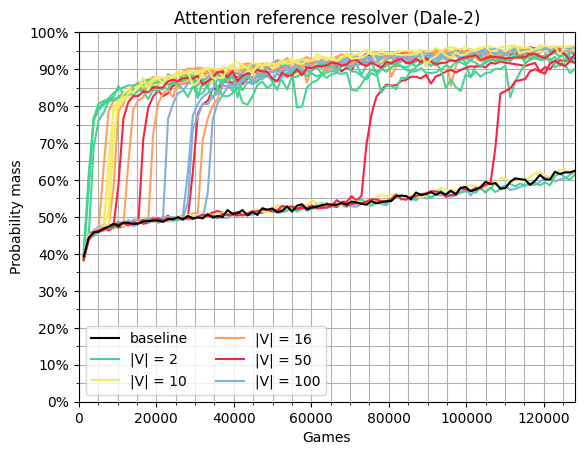
\includegraphics[width=0.3\linewidth]{figures/learning-curve_attention-predictor_dale-2_vocab-size.png}
    \label{fig:learning-curve_attention-predictor_dale-2_vocab-size}
  }
  \subfigure['Dale-5' dataset]{
    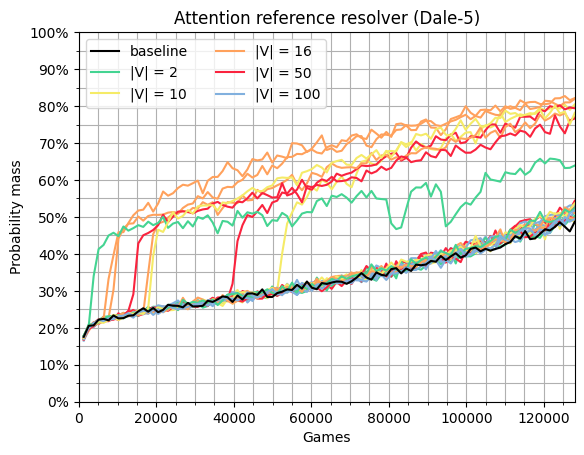
\includegraphics[width=0.3\linewidth]{figures/learning-curve_attention-predictor_dale-5_vocab-size.png}
    \label{fig:learning-curve_attention-predictor_dale-5_vocab-size}
  }
  \subfigure['CLEVR color' dataset]{
    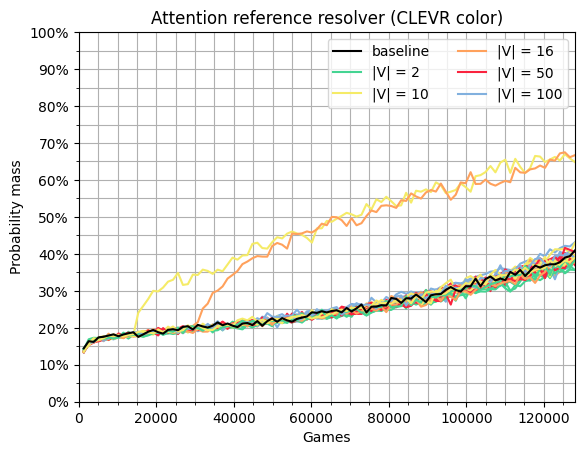
\includegraphics[width=0.3\linewidth]{figures/learning-curve_attention-predictor_colour_vocab-size.png}
    \label{fig:learning-curve_attention-predictor_colour_vocab-size}
  }
  \caption{Learning curves of all language games on each dataset. The colors correspond to different vocabulary sizes $|V|$. The baseline is marked in black.}
  \label{fig:learning-curves_attention-predictor}
\end{figure*}

Our dataset conists of images of contrasting scenes and objects.  The
scenes are generated from an adapted code that was used to generate
the \textbf{CLEVR dataset}. Instead of focusing on compositional
properties of descriptions, we generate scenes with increasing
complexity and control over object attributes, inspired by \citep{Dale1995}, but we
used the \textbf{feature hirerachy} to generate visual scenes rather
than generate descriptions. We create the following datasets:
% To systematically study emergent communication, the authors extend the
% \textbf{CLEVR dataset}---a synthetic dataset designed for visual
% reasoning. They create three new datasets with increasing complexity and
% control over object attributes:

In \textbf{CLEVR color}, the target object is uniquely identifiable by
\textbf{color alone}. All distractors share the same shape and size as
the target. %, making color the only distinguishing feature. This setup is
% relatively simple and
This allows the study of how agents learn to use a
single attribute for reference.
%
\textbf{Dale-2}
% Inspired by the Dale-Reiter algorithm, this dataset
includes \textbf{one
  target and one distractor}. The target is uniquely identifiable by a
minimal combination of attributes (color, shape, size). This setup introduces more
variability and requires agents to learn which attributes are most
informative in each context.
%
\textbf{Dale-5} increases complexity by including \textbf{one target and
  four distractors}. The target may share multiple attributes with
different distractors, requiring more complex referring expressions.
This setup closely mirrors real-world scenarios where objects often
share overlapping features.
%
Each dataset contains 10,000 images, with up to 10 non-overlapping
objects per image. The images are $480\times 320$ pixels, and objects are placed
to ensure visibility and spatial separation.

% \textbf{3.1 Image Processing}

Images are processed using a \textbf{ResNet-101} model, followed by two
convolutional layers with ReLU activations. These layers reduce the
feature maps to 128 channels.


\section{Experiments}
The games are set up through the \textbf{EGG framework} \citep{Kharitonov2019} that allows communication through a discrete channel with an LSTM.
Backpropagation is enabled through \textbf{Gumbel-Softmax  relaxation}.

The receiver's task is to predict a $3 \times 3$ region around the target object in a $14 \times 14$ grid over the image (see Appendix \ref{app:architecture}).
The model outputs a probability distribution over all regions, and performance is measured by the \textbf{probability mass} assigned to the correct region.
The sender encodes bounding boxes of all objects and passes them through an LSTM to generate a message.
The receiver decodes the message and combines it with its own visual representation of the scene to predict the target region.
The receiver does not have enough information to solve the task on its own.
A total of 128.000 games are played.
Furthermore, we allow different message lengths vocabulary sizes.
All results are compared to a baseline in which the sender is generating random messages.

On the 'Dale-2' dataset, almost all configurations outperform the baseline, with top-configurations achieving over 96\% probability mass (see Appendix \ref{app:results}).
Message length primarily influences performance, with $n \in \{3,4\}$ yielding consistent results.
While $n=6$ configurations can succeed, they are less reliable.
Vocabulary size shows less impact, though $|V|=2$ performs slightly worse.
No clear correlation between $n$ and $|V|$ emerges.
On the 'Dale-5' dataset, only 8 out of 30 configurations beat the baseline.
Best models reach 84\%, but many struggle due to the increased complexity.
Shorter messages ($n \in \{2,3\}$) and medium vocabularies ($|V| \in \{10,16,50\}$) are most effective.
The increased number of distractors complicates the task: objects share more attributes, requiring more complex descriptions, and their spatial proximity can lead to confusion in region identification.
Performance is weakest on the 'CLEVR color' dataset, with only two configurations beating the baseline (64-67\%), both using medium message lengths ($n \in \{3,4\}$) and vocabularies ($|V| \in \{10,16\}$).
Notably, short messages ($n=2$) often mislead the receiver.
The presence of up to 10 objects increases the likelihood of focusing on incorrect targets.

\section{Findings and future directions}

Our study shows (i) that \textbf{emergent communication is possible}
and in the studied environments and network configurations but (ii)
\textbf{scene complexity} significantly affects learning. More
distractors and overlapping attributes make it harder for agents to
learn effective communication. (iii) \textbf{Medium-sized vocabularies
  and message lengths} strike the best balance between expressiveness
and learnability.
% \textbf{Natural language grounding} improves performance, especially in complex scenes. %% % SD 2025-07-19 09:48:09 +0200: Not sure where it got this from!
(iv) \textbf{Attribute difficulty}: shape is easiest to learn,
followed by color, with size being the hardest. This mirrors findings
in human cognition and suggests that (v) \textbf{neural networks may
  benefit from similar inductive biases}. The findings suggest that
that successful language-vision models must go beyond mere observation
of pixels and words where such biases would be provided. They must
incorporate \textbf{structured representations}, \textbf{attention
  mechanisms}, and \textbf{pragmatic reasoning} to handle real-world
complexity.

% \textbf{8. Future Directions}

% The paper outlines several avenues for future research:

% \begin{itemize}
% \tightlist
% \item
%   \textbf{Linguistic analysis of emergent languages}: Do they exhibit
%   compositionality, syntax, or other properties of natural language?
% \item
%   \textbf{Transfer learning}: Can agents trained in synthetic
%   environments generalize to real-world data?
% \item
%   \textbf{Pragmatic reasoning}: How can models learn to select the most
%   informative attributes, as humans do?
% \item
%   \textbf{Interactive learning}: Can agents learn more effectively
%   through dialogue and feedback?
% \end{itemize}

% These directions aim to bridge the gap between synthetic experiments and
% real-world applications, ultimately leading to more robust and
% interpretable AI systems.


% Bibliography entries for the entire Anthology, followed by custom entries
%\bibliography{anthology,custom}
% Custom bibliography entries only
\bibliography{custom}

\appendix

\section{Architecture of the language game}
\label{app:architecture}

\begin{figure}[ht!]
  \centering
  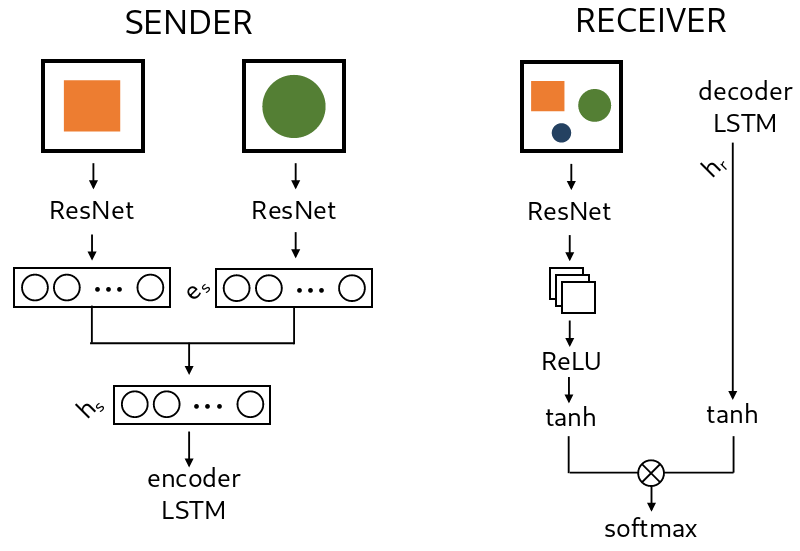
\includegraphics[width=0.7\linewidth]{figures/arch_attention_predictor_game.png}
  \caption{Simplified architecture of the attention predictor game.}
  \label{fig:attention_predictor_game_architecture}
\end{figure}


\section{Results}
\label{app:results}

\begin{table}[ht!]
  \footnotesize
  \centering
  \begin{tabular}{cc|c|c|c}
    \toprule
                                  &           & \multicolumn{1}{c}{\textbf{Dale-2}} & \multicolumn{1}{c}{\textbf{Dale-5}} & \multicolumn{1}{c}{\textbf{color}} \\  \cmidrule(lr){3-3}\cmidrule(lr){4-4}\cmidrule(lr){5-5}
    $n$                           & $|V|$     & \textbf{$P$ mass}                   & \textbf{$P$ mass}                   & \textbf{$P$ mass}                  \\\midrule
    \multicolumn{2}{c|}{baseline} & {62,16\%} & {49,61\%}                           & {41,68\%}                                                                \\\midrule
    {2}                           & {2}       & {92,27\%}                           & \textcolor{red}{52,15\%}            & \textcolor{red}{33,64\%}           \\
    {3}                           & {2}       & {94,52\%}                           & \textcolor{red}{51,97\%}            & \textcolor{red}{37,09\%}           \\
    {4}                           & {2}       & {89,15\%}                           & \textcolor{red}{51,98\%}            & \textcolor{red}{39,68\%}           \\
    {6}                           & {2}       & \textcolor{red}{59,68\%}            & \textcolor{red}{53,57\%}            & \textcolor{red}{38,43\%}           \\
    {2}                           & {10}      & \textbf{96,16\%}                    & {80,26\%}                           & \textcolor{red}{36,53\%}           \\
    {3}                           & {10}      & {94,9\%}                            & \textcolor{red}{53,47\%}            & \textcolor{red}{38,24\%}           \\
    {2}                           & {16}      & {95,84\%}                           & \textbf{84,03\%}                    & \textcolor{red}{39,65\%}           \\
    {4}                           & {10}      & \textbf{96,08\%}                    & \textcolor{red}{48,03\%}            & \textbf{64,31\%}                   \\
    {3}                           & {16}      & {94,59\%}                           & \textbf{81,46\%}                    & \textbf{67,88\%}                   \\
    {6}                           & {10}      & \textcolor{red}{63,46\%}            & \textbf{82,12\%}                    & \textcolor{red}{40,11\%}           \\
    {4}                           & {16}      & {94,14\%}                           & \textcolor{red}{49,81\%}            & \textcolor{red}{40,84\%}           \\
    {6}                           & {16}      & {95,86\%}                           & \textcolor{red}{50,71\%}            & \textcolor{red}{40,61\%}           \\
    {2}                           & {50}      & {93,78\%}                           & \textcolor{red}{52,24\%}            & \textcolor{red}{39,56\%}           \\
    {3}                           & {50}      & {93,88\%}                           & {79,65\%}                           & \textcolor{red}{40,36\%}           \\
    {2}                           & {100}     & {92,43\%}                           & \textcolor{red}{53,23\%}            & \textcolor{red}{37,68\%}           \\
    {4}                           & {50}      & \textbf{96,24\%}                    & \textcolor{red}{48,79\%}            & \textcolor{red}{43,61\%}           \\
    {3}                           & {100}     & {95,25\%}                           & \textcolor{red}{48,52\%}            & \textcolor{red}{42,55\%}           \\
    {6}                           & {50}      & {91,27\%}                           & \textcolor{red}{52,55\%}            & \textcolor{red}{40,21\%}           \\
    {4}                           & {100}     & {95,55\%}                           & \textcolor{red}{49,65\%}            & \textcolor{red}{42,85\%}           \\
    {6}                           & {100}     & \textcolor{red}{60,27\%}            & \textcolor{red}{46,92\%}            & \textcolor{red}{41,98\%}           \\
    \bottomrule
  \end{tabular}
  \caption{Probability masses of the attention reference resolver after 128.000 games: $n$ are different maximum message lengths and $|V|$ are different vocabulary sizes. Results in red didn't pass the baseline. The results are sorted by the product of $n$ and $|V|$ which corresponds to available space for the message. The best results are achieved with a medium-sized message space across all datasets.}
  \label{tab:results:attention-reference-resolver-game}
\end{table}

\end{document}

%%% Local Variables:
%%% mode: latex
%%% mode: flyspell
%%% TeX-master: t
%%% TeX-PDF-mode: t
%%% coding: utf-8
%%% ispell-local-dictionary: "british"
%%% End:
